\documentclass[twocolumn]{aastex62}

\usepackage{graphicx}
\usepackage{url}
\usepackage{hyperref}


%% Reintroduced the \received and \accepted commands from AASTeX v5.2
\received{...}
\revised{...}
\accepted{...}
%% Command to document which AAS Journal the manuscript was submitted to.
%% Adds "Submitted to " the argument.
%\submitjournal{ApJ}


\begin{document}

\title{Spatially resolved velocity structure in jets of DF Tau and UY Aur A}


\correspondingauthor{Anastasiia V Uvarova}
\email{avu@mit.edu}

\author{Anastasiia V Uvarova}
\affil{MIT, Kavli Institute for Astrophysics and Space Research, 77 Massachusetts Avenue, Cambridge, MA 02139, USA}

\author[0000-0003-4243-2840]{Hans Moritz G\"unther}
\affil{MIT, Kavli Institute for Astrophysics and Space Research, 77 Massachusetts Avenue, Cambridge, MA 02139, USA}

\author{D. A. Principe}
\affil{MIT, Kavli Institute for Astrophysics and Space Research, 77 Massachusetts Avenue, Cambridge, MA 02139, USA}

\author{P. C. Schneider}
\affil{Hamburger Sternwarte, Universit\"at Hamburg, Gojenbergsweg 112, 21029, Hamburg, Germany}

\begin{abstract}
Young stars accrete mass and angular momentum from their circumstellar
disks. Some of them also drive outflows, which can be distinguished in
optical forbidden emission lines (FELs). We analyze a sample of binary
T Tauri stars observed with long-slit spectroscopy by the Hubble space
telescope, searching for spatially resolved outflows. We detect resolved [O~{\sc i}] emission in two cases out of twenty one. In DF Tau we resolve high and medium velocity outflows in a jet and counterjet out to 60~au. The outflows are accelerated within the inner 12~au and retain a constant speed thereafter. In UY~Aur, we detect a blue- and a red-shifted outflow from UY~Aur~A, as well as a blue-shifted jet from UY~Aur~B. All of these features have been seen in [Fe~{\sc ii}] with data taken ten years apart, indicating that the underlying outflow pattern is stable on these timescales.
\end{abstract}%


\section{Introduction}

Star formation occurs when large clouds of gas and dust collapse due to
gravity. The clouds are inhomogeneous in density and they fragment into
smaller structures, where the center of each collapsing sub-cloud may
become a star or system of stars. Very few of the resulting stars are
massive and hot. By far the largest number will evolve into late-type
stars with spectral types in the M-F range. Most stars are members of a binary or multiple multiple systems \citep[see e.g.\ review by][]{2007prpl.conf..379D}.
The infalling envelope
flattens to a circumstellar disk, making the stars visible in the
optical. Low-mass stars in this stage are called classical T Tauri stars
(CTTS). For a few Myrs, planet formation can take place before the disk
disperses. For binaries or higher-order multiple systems, the disk can
belong to an individual star or surround a close binary pair depending
on the mass and separation of the components.

Mass is accreted through these disks onto the stars. However,
conservation of angular momentum demands that some mass is ejected and
carries away the angular momentum accreted through
the disk. Mass
loss occurs through wide-angle disk winds, but in some systems we 
also see highly collimated jets. These jets typically have an onion-like
structure with a fast component at the center surrounded by increasingly
slower and less collimated components further
out \citep{2000ApJ...537L..49B}. Forbidden optical emission lines (FELs) are a
good way to find and study such jets, since the stellar photosphere and
the accretion shock are too dense to contribute significantly to the emission. If a
jet is detected in several emission lines, line ratios can be used to
calculate density and ionization fraction of emission components in the
jet with typical densities in the range~$10^3-10^5\;\mathrm{cm}^{-3}$
\citep[e.g.][]{1999A&A...342..717B,2000A&A...356L..41L,2013A&A...550L...1S}. In turn
the density and the velocity give mass loss rates. Different outflow
components show different velocities. For example, in the well-studied
CTTS DG Tau~\citet{2013A&A...550L...1S} find [O~{\sc i}] in a low-velocity
component (LVC, about 60~km~s$^{-1}$) which can be detected as
close as 15~au from the star and a medium-velocity component (MVC, about
130~km~s$^{-1}$) first detected at about 50 au from the source. The MVC in DG~Tau
slows down at larger distances. While a single spectrum is sufficient to
detect the presence of a FEL, spatially resolved data is nessesary to study
how outflows accelerate and decelerate. In this work, we reanalyze
archival data from the Hubble Space Telescope (HST) Program ID 7310 to
search for FELs that are spatially resolved.

In section~\ref{sect:obs} we describe the observations and the data reduction. Section~\ref{sect:results} presents our immediate results. We discuss the resolved emission from DF~Tau and UY~Aur in section~\ref{sect:discussion} and end with a short summary in section~\ref{Sect:summary}.

\section{Observations and data reduction}
\label{sect:obs}

\begin{table*}
\cpation{Log of observations\label{tab:obs}}
\begin{center}
\begin{tabular}{cccccc}
\hline\hline
OBSID G750L & OBSID G750M & Target & Observation Date & Aperture & Position angle (deg) \\
\hline
o55101010& o55101020 & FO TAU & 1999-10-17 & 52X0.2 & 50.15 \\

%o55101020 & FOTAU & 1999-10-17 & 52X0.2 & 50.15 \\

o55102010& o55102020 & DD TAU & 1999-09-05 & 52X0.5 & 64.54 \\

%o55102020 & DDTAU & 1999-09-05 & 52X0.5 & 64.54 \\

o55104010& o55104020 & UZ TAU-W & 1999-11-02 & 52X0.2 & 52.54 \\

%o55104020 & UZTAU-W & 1999-11-02 & 52X0.2 & 52.54 \\

o55105010& o55105020 & LKCA 7 & 1999-01-25 & 52X0.2 & 250.0 \\

%o55105020 & LKCA7 & 1999-01-25 & 52X0.2 & 250.0 \\

o55106010& o55106020 & LKHA 332 & 1998-12-23 & 52X0.2 & 251.0 \\

%o55106020 & LKHA332 & 1998-12-23 & 52X0.2 & 251.0 \\

o55107010& o55107020 & UY AUR & 1998-12-25 & 52X0.2 & 271.0 \\

%o55107020 & UYAUR & 1998-12-25 & 52X0.2 & 271.0 \\

o55108010& o55108020 & 040047+2603W & 1998-12-04 & 52X0.2 & 272.0 \\

%o55108020 & 040047+2603W & 1998-12-04 & 52X0.2 & 272.0 \\

o55109010& o55109020 & FQ TAU & 1998-12-05 & 52X0.5 & 303.0 \\

%o55109020 & FQTAU & 1998-12-05 & 52X0.5 & 303.0 \\

o55110010& o55110020  & FS TAU & 2000-12-13 & 52X0.2 & 309.0 \\

%o55110020 & FSTAU & 2000-12-13 & 52X0.2 & 309.0 \\

o55111010& o55111020 & HARO6-28 & 1998-12-02 & 52X0.2 & 290.1 \\

%o55111020 & HARO6-28 & 1998-12-02 & 52X0.2 & 290.1 \\

o55112010& o55112020 & LKHA332G2 & 1998-12-12 & 52X0.5 & 269.4 \\

%o55112020 & LKHA332G2 & 1998-12-12 & 52X0.5 & 269.4 \\

o55113010& o55113020 & 040142+2150 & 1998-12-01 & 52X0.2 & 289.0 \\

%o55113020 & 040142+2150 & 1998-12-01 & 52X0.2 & 289.0 \\

o55114010& o55114020 & IS TAU & 2000-12-03 & 52X0.2 & 317.0 \\

%o55114020 & ISTAU & 2000-12-03 & 52X0.2 & 317.0 \\

o55115010& o55115020 & FV TAU & 2000-12-03 & 52X0.5 & 322.4 \\

%o55115020 & FVTAU & 2000-12-03 & 52X0.5 & 322.4 \\

o55116010& o55116020 & FV TAU-C & 1998-12-02 & 52X0.2 & 337.0 \\

%o55116020 & FVTAU-C & 1998-12-02 & 52X0.2 & 337.0 \\

o55117010& o55117020 & GH TAU & 2000-12-01 & 52X0.2 & 350.8 \\

%o55117020 & GHTAU & 2000-12-01 & 52X0.2 & 350.8 \\

o55118010& o55118020 & LKHA 331 & 1999-10-08 & 36X0.6P45 & 100.0 \\

%o55118020 & LKHA331 & 1999-10-08 & 36X0.6P45 & 100.0 \\

o55119010 & o55119020 & UZ TAU-W-OFF & 2000-09-04 & 52X0.5 & 64.79 \\

%o55119020 & UZTAU-W-OFF & 2000-09-04 & 52X0.5 & 64.79 \\

o55120010& o55120020 & DF TAU & 1998-11-26 & 52X0.2 & 18.04 \\

%o55120020 & DFTAU & 1998-11-26 & 52X0.2 & 18.04 \\

o55121010& o55121020 & XZ TAU & 2000-12-02 & 52X0.2 & 194.1 \\

%o55121020 & XZTAU & 2000-12-02 & 52X0.2 & 194.1 \\

o55122010& o55122020 & V807 TAU & 1998-11-30 & 52X0.2 & 19.03 \\

%o55122020 & V807TAU & 1998-11-30 & 52X0.2 & 19.03 \\
\hline
\end{tabular}
\end{center}
\end{table*}



Hubble Space Telescope (HST) Program ID 7310 targets binary T Tauri
stars with long-slit spectroscopy using the Space Telescope Imaging
Spectrograph (STIS). The long slit is always oriented such that both
components of the binary are observed. \citet{2003ApJ...583..334H} analyze the
spectra of both stellar components to determine stellar properties and
accretion diagnostics. In this work, we aim to spatially resolve the
emission in FELs along the slit, i.e. jets, around those stars.

Table~\ref{tab:obs} lists the observations presented in this paper. The observations for each of the stars were taken using two different gratings: G750L and G750M, with central wavelengths of 7751~\AA{} and 6252~\AA{} with exposure times of 360~s and 1080~s respectively. The observations were consecutive in the same orbit. Position angles are measured East of North. \citet{2003ApJ...583..334H} lists properties (including binary separation and position angle, but also derived properties like stellar mass and accretion) in tables for all targets.

Our analysis begins from the pipeline reduced
2-dimensional~\texttt{sx2} files; these files have one spectral axis and
one spatial axis for the coordinate along the slit. For each wavelength
in~\texttt{sx2} we fit a single Gaussian to approximate the spatial flux distribution (dominated by the point-spread function (PSF) of the star), taking into account regions
flagged for data quality by the pipeline. While this does not capture
all features of the instrumental PSF, it describes the signal close to the
peak of the emission well and allows a numerically stable fit of the
position of the peak.

The measured peak position  of the Gaussian changes with
wavelength in a smooth manner, both due to minor misalignment between slit and CCD as well as due to the distortion corrections done in the data
pipeline. The scatter in the fit results can be
taken as an estimate of uncertainty of our fits.
If both components of the binary system are within a few arcseconds of
each other, a fit using two Gaussians is performed. All fits are
visually inspected. 

We search for changes
of the fitted position of the Gaussian, i.e.\ changes in the mean
position of the emission around the wavelength of forbidden emission
lines (FELs, see table~\ref{tab:searchedlines}). Limiting our search in this way reduces the
rate of false-positives. Since FELs can only be formed in low-density
environments, they are tracers of outflows and cannot originate on the
star.

We show those data as position-velocity-diagrams (PVD) in Fig~\ref{fig:DFTau}, where the
origin of the spatial coordinate is set on the position of one of the stars and the velocity is derived from the radial velocity  of
a stellar feature. In a PVD, resolved
FEL emission is seen as~ a bulge in the vicinity of the rest wavelength
in the emission line, if the direction of the slit roughly aligns with
the direction of the jet.


%\textbf{TABLE WITH THE
%LINES~\url{http://classic.sdss.org/dr6/algorithms/linestable.html}}

\begin{table}
\caption{{Lines searched for spatial extension\label{tab:searchedlines}}}
\begin{center}
\begin{tabular}{cc}
\hline\hline
line & wavelength [\AA] \\
\hline
[O I] & 6302.0\\{}
[O I] & 6365.5\\{}
[O III] & 5008.240\\{}
[O III] & 4960.295\\{}
[O III] & 4364.436\\{}
[N II] & 6549.86\\{}
[N II] & 6585.27\\{}
[S II] & 6718.29\\{}
[S II] & 6732.67\\
\hline
\end{tabular}
\end{center}
\end{table}


To investigate the jets in these selected stars we subtract the contribution of the stellar continuum similar to the method of \citep{2013A&A...550L...1S}: For every row of in the image (in the dispersion direction) we select a region on interest centered on the position of the FEL (15 pixels wide for the G750M data and 2 pixels wide in the G750L data, where the FELS are not resolved). Assuming that the PSF is only slowly changing with wavelength and that the stellar emission is mostly continuum, we fit a second degree polynomial to the data to the left and right of the FEL. The region used for the fit is 10 pixels wide in the G750M data and 5 pixels wide in the G750L data. We subtract the value of the polynomial for every row of data in the FEL region. The remaining images should display signatures of jets if there are any, and can be used to examine jet profiles and intensities. This work is focused on features in the vicinity of the oxygen lines and thus we selected a
region around these lines and performed the subtraction.

\section{Results}
\label{sect:results}

\subsection{Significantly extended FELs}
We detected significantly extended emission only in two out of 21 objects, DF~Tau and UY~Aur. In both cases, the extension is seen in the [O~{\sc i}] lines, but is not significantly detected in any other FEL. \citet{2003ApJ...583..334H} already noted that the on-source [O~{\sc i}] line profile shows different kinematic components for both components of DF~Tau and the primary of UY~Aur, while all other targets have simple [O~{\sc i}] line profiles. \citet{2003ApJ...583..334H} also discuss \object{FS Tau} p where they note an [O~{\sc i}] line that appears spatially extended. FS~Tau shows an extension in our processing, however, that is due entirely due to the signal from a single pixel, which is flagged as TBD by the data processing pipeline. No spatial extension is seen after removing that spurious signal.

The PVDs for FELs detected as extended are shown in figures~\ref{fig:DFTau} and \ref{fig:UYAur}. 

\subsubsection{DF Tau}
\begin{figure}
\begin{center}
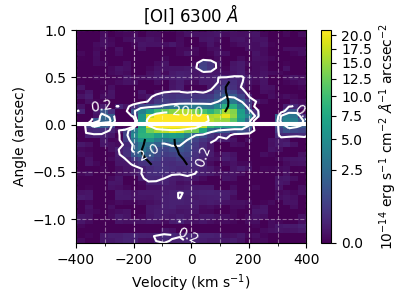
\includegraphics[width=0.49\textwidth]{DF_6300.png}
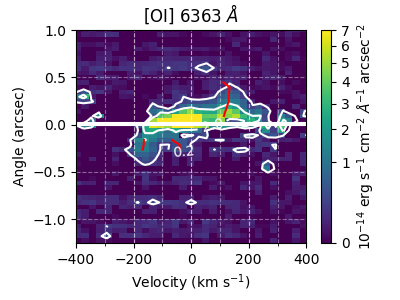
\includegraphics[width=0.49\textwidth]{DF_6363.png}
\caption{Position velocity diagrams (PVD) for the subtracted images
of DF Tau; the two components of the binary are not resolved. The x-axis
shows the velocity with respect to the feature rest wavelength in the
velocity frame of the star and the y-axis is the distance along the slit. The
continuum emission from the two stars has been subtracted. The color scale is chosen to highlight faint emission features; negative values or brighter fluxes are shown as purple or yellow, respectively. Contours show flux densities in $10^{-14}$~erg~s$^{-1}$~cm$^{-2}$~\AA{}$^{-1}$~arcsec$^{-2}$.
\textbf{The black lines highlight the jet emission. They were plotted by doing the Gaussian fit to each of the rows in the vicinity of the jet emission and taking the mean of those fits. The uncertainty of the resulting fits lies within the line thickness}
\label{fig:DFTau}}
\end{center}
\end{figure}
The [O~{\sc i}] PVD for DF Tau is shown in figure~\ref{fig:DFTau}
corrected for the stellar radial velocity from \citet{2006AstL...32..759G}.
Both sides of the jet can be traced to a similar distance. The observed velocity of the HVC of the approaching jet is about -150 to -200~km~s$^{-1}$. Since we do not know the inclination angle with respect to the line-of-sight observed velocities are lower boundaries to the true jet speed. There are indications for a MVC around -50~km~s$^{-1}$), but the emission is weaker than the HVC. We also see the red-shifted counter jet at a velocity around +150~km~s$^{-1}$ and a single emission feature at 50~km~s$^{-1}$, located about 0\farcs6 from the star (72~au projected on the plane of the sky). The HVC of jet and counterjet is seen to about 0\farcs5 (60~au). All those features are seen in both [O~{\sc i}] lines, which gives us confidence that even the weaker features are real detections and not just background fluctuations.

Within about 0\farcs1 from the star (12~au) the velocity of the fasted outflow component of both jet and counterjet seems to increase, as the peak of the emission moves towards larger velocities in this region. No change in velocity is seen at larger radii.

\subsubsection{UY Aur}
\begin{figure}[h!]
\begin{center}
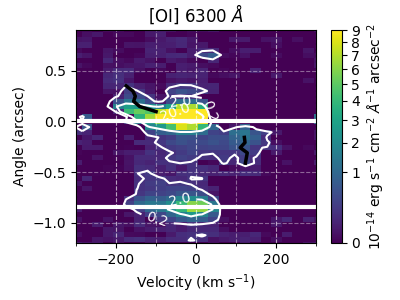
\includegraphics[width=0.49\textwidth]{UY_Aur_6300.png}
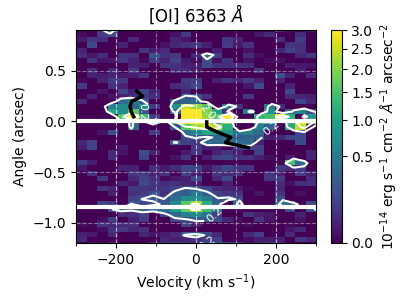
\includegraphics[width=0.49\textwidth]{UY_Aur_6363.png}
\caption{Position velocity diagrams for subtracted
image of UY Aur; The x-axis shows the velocity with respect to the
feature rest wavelength in the velocity frame of the star UY Aur
A and the y-axis the distance along the slit. Both components of the UY Aur AB binary are shown.
\label{fig:UYAur}
}
\end{center}
\end{figure}
We take the radial velocities from~\citet{2012ApJ...745..119N} for UY~Aur and show a PVD in figure~\ref{fig:UYAur}. There is a HVC around -150 to -200~km~s${-1}$ and a MVC around -50~km~s${-1}$. Both are visible to about 0\farcs25 (40~au) in the figure. At [O~{\sc i}]~6302\AA{}, three emission components are seen between the two stars. Two of them seem to originate on UY~Aur A (the upper star in the figure) and have velocities around -50 and +150~km~s$^{-1}$. In [O~{\sc i}]~6366\AA{} the signal is lower. It is thus not clear, if these are two separate flow components or if these velocities represent just the extreme ends of a kinematic distribution that spans from red- to blue-shifted velocities. In [O~{\sc i}]~6302\AA{} there is a third component, apparently origination from UY~Aur~B with a velocity about -100~km~s$^{-1}$, but no significant emission is seen in [O~{\sc i}]~6366\AA{} at this location, so we regard this detection as tentative.


\subsection{Upper limits}
The [O~{\sc i}] lines are the only FELs from table~\ref{tab:searchedlines} that fall in the wavelength range of the G750M gratings. We attempt to detect other lines in the G750L data using our subtraction procedure but cannot perform this measurement for the [N~{\sc ii}] lines, because they are too close to the H$\alpha$ line. The [O~{\sc i}] lines are kinematically unresolved, but fluxes are consistent with what is seen in G750M gratings. We inspected figures analogous to figure~\ref{fig:DFTau} and \ref{fig:UYAur} for for several regions free of FELs to determine the average noise. We conclude that the [S~{\sc ii}] lines are not detected for any source from table~\ref{tab:obs}. Line-free regions and the [S~{\sc ii}] lines show residuals that decline with distance from the stars with an average of $10^{-14}$~erg~s$^{-1}$~\AA{}$^{-1}$~arcsec$^{-2}$ at 0\farcs2 and 0.05$\times10^{-14}$~erg~s$^{-1}$~\AA{}$^{-1}$~arcsec$^{-2}$ at 0\farcs5. Thus, we conclude that the [O~{\sc i}] lines are at least 3-5 times stronger than [S~{\sc ii}] in DF~Tau and at least two times stronger in UY~Aur. We also checked H$\alpha$ for extension, but did not find extended emission that could indicate a presence of a jet. 

\subsection{Mass loss rates}
With some assumptions on the physical conditions in the jet, we can estimate the total mass loss rate in the resolved outflow components. Following \citet{1994ApJ...436..125H}, we take a plasma with solar abundances emitting close to the peak formation temperature of the [O~{\sc i}] lines a. To do so, we need to make assumptions. Any jet components that are located outside the
aperture, so hot that oxygen is ionized or so cool that that  [O~{\sc i}] 6300\AA{} is not excited, or with densities above the critical density for [O~{\sc i}] ($10^6$~cm$^{-3}$), are not accounted for in this estimate. Thus, the estimate is a lower limit in the total mass flux in the jet. We use
\begin{eqnarray}
\dot M  & = & 5.95\times10^{-8} \left(\frac{n_e}{10^3\textnormal{ cm}^{-3}}\right)^{-1}\left(\frac{L_{6300}}{10^{-4} L_{\sun}}\right) \nonumber\\
 & & \times \left(\frac{v_{sky}}{100\textnormal{ km s}^{-1}}\right)\left(\frac{l_{sky}}{10^{16}\textnormal{ cm}}\right)^{-1} M_{\sun} \textnormal{ yr}^{-1} \ ,
\end{eqnarray}
which is eqn.~10 from \citet{1994ApJ...436..125H}. Alternatively, a very similar calculation can be done using the [S~{\sc ii}] lines. If they are within the high-density limit ($>10^4$~cm$^{-3}$), then the formula does not depend on the density in the knot \citep[][eqn A.10]{1995ApJ...452..736H}: 
\begin{eqnarray}
\dot M  & = & 4.5\times10^{-9} \left(\frac{L_{6731}}{10^{-4} L_{\sun}}\right)\left(\frac{v_{sky}}{100\textnormal{ km s}^{-1}}\right) \nonumber\\
 & & \times \left(\frac{l_{sky}}{10^{16}\textnormal{ cm}}\right)^{-1} M_{\sun} \textnormal{ yr}^{-1} \; .
\end{eqnarray}


\section{Discussion}
\label{sect:discussion}
We detect spatially extended emission in about 10\% of observations. In the remaining objects, jets must be either weak, not present, or simply not aligned with the slit in the observations. However, the fact that the two objects with extended emission are also the two objects that show multiple kinematic components in the [O~{\sc i}] emission lines \citet{2003ApJ...583..334H}, 

We compare our detections to other observations of the same jets in the literature to put the properties of these jets into context.

\subsection{DF Tau}

\object{DF Tau} is located at a distance of $125\pm6$~pc
\citep{2016A&A...595A...1G,2018A&A...616A...1G}. It is a binary composed of two
equal mass M2 dwarfs separated by 0.1~arcsec (12.5~au). The primary shows an
infrared excess in its spectral energy distribution (SED), indicating the
presence of a disk, and signatures of accretion, while the secondary seems to
be devoid of circumstellar material \citep{2017ApJ...845..161A}, yet
\citet{2003ApJ...583..334H} determine equal accretion rates of $\dot M=10^{-7}$~M$_{\sun}$~yr$^{-1}$ for both stars from spectral fitting.
\citet{2004ApJ...609..261H} observed the jet of DF Tau with low-resolution slitless spectroscopy with STIS. They detect a jet and counterjet at a
position angle of 127~degrees, but the binary is not resolved and it was unclear at the time which star was the origin of which outflow component. Given the absence of circumstellar material around the secondary component, it seems very likely now that we are looking at a bipolar jet launched from the primary star. 

In the observations presented here, the position angle of the slit was 153~degrees, only 26~degrees from the jet axis. This means that for distances beyond about 0\farcs5, a well-collimated outflow would not be visible any longer in our images because it reaches the edge of the 0\farcs2 wide slit and indeed little signal is detected at larger distances from the star. The LVC seen at 0\farcs6 must therefore be part of a larger, possibly less collimated, structure. When the emission is not centered in the slit, the wavelength scale is not accurate. However, a slit half-width of 0\farcs1 corresponds to only 2 pixels (about 50~km~s$^{-1}$). Given the size of the PSF, even a source located on the edge of the slit would be detected in several pixels, so the maximal velocity shift that can be explained by the emission not being centered in the slit is about $\pm30$~km~s${-1}$.

This data was taken about one and two years before the two slitless exposures of \citet{2004ApJ...609..261H} respectively. We trace the jet out to slightly larger distances and resolve a HVC and MVC on both sides of the jet, while the slitless data does not allow a velocity measurement.


\subsection{UY Aur}

\object{UY Aur} is  located at a distance of $156\pm2$~pc \citep{2016A&A...595A...1G,2018A&A...616A...1G}. It again is a binary system with two components of similar mass \citep[M0 and M2, see][]{2003ApJ...583..334H}. \citet{2003ApJ...583..334H} determine very similar mass accretion rates around $\dot M=2\times10^{-8}$~M$_{\sun}$~yr$^{-1}$.
UY~Aur~A has a disk resolved by ALMA with a position angle of $177\pm11$~degrees and an inclination of $56\pm16$ degrees \citep{2014ApJ...784...62A}. FELs in a jet were observed in 1988 by \citet{1997A&AS..126..437H} in ground-based observations with a position angle around 40~degrees. They trace the emission out to several arcsec in [O~{\sc i}]~6300~\AA{}. The spectral and spatial resolution of their data is not as good as what we present here, but it traces the jet out to larger distances. Their data indicate the presence of different emission components ranging from -240~km~s$^{-1}$ in the approaching jet to +180~km~s$^{-1}$ in the receding jet. More recently \citet{2014ApJ...786...63P} performed adaptive-optics observations with an integral field unit (IFU) in the IR and they obtain detailed images in the [Fe~{\sc ii}] $\lambda$1.257~$\mu$m line. They detect blue-shifted emission in a circular region around the primary as well as in a ``bridge'' that connects the primary and the secondary (offset by about 0\farcs2 to the north from the direct line connecting the primary and the secondary); redshifted emission is seen close to the primary on the side that faces towards the secondary as well as in the ``bridge'' region. Together with the absorption features observed in the stellar spectra, this suggests a geometry where the primary has a wide-angle, fast wind on both sides and a more collimated, red-shifted jet on the far side of the disk, in the direction of the secondary. The secondary does not have a wide-angle wind in [Fe~{\sc ii}] but only a collimated jet. In the ``bridge'' region we see the red-shifted jet of the primary and the blue-shifted jet of the secondary projected onto the same area of the sky.

The long-slit in our data contains both stars of the binary and overlaps the ``bridge'' region in between. The slit is 0\farcs2 wide, so it contains some of the flux in the ``bridge'', but not the peak of the flux distribution. Looking just at the region covered by our slit, we see remarkably similar emission in [O~{\sc i}] compared with the [Fe~{\sc ii}] observations of \citet{2014ApJ...786...63P}. We also have indications for a fast, blue-shifted outflow ``above'' UY Aur~A and we see both red-and blue-shfited emission in the ``bridge'' region, again with velocities similar to those seen in [Fe~{\sc ii}]. Given that the data from \citet{1997A&AS..126..437H} was taken in 1988, this data in 1998, and the \citet{2014ApJ...786...63P} data in 2007 and that the feature with a velocity of 200~km~s$^{-1}$ would move about 3\arcsec{} on the sky in ten years, this indicates all features seen represent stable outflow patterns. This includes the blue-shifted outflow from UY~Aur~A, interpreted as a fast, wide angle wind by \citet{2014ApJ...786...63P}, the red-shifted outflow from UY Aur~A (interpreted as a fast, wide-angle wind, too), and the blue-shifted outflow from UY~Aur~B (identified as a jet).

\subsection{Comparison to other jets}
The mass accretion rate measured in DF Tau is about five times stronger than in UY~Aur \citet{2003ApJ...583..334H} and \textbf{check numbers with Ana: consistent with this the resolved [O~{\sc i}] emission is also about XXX stronger.} 
\textbf{HMG: Should there be a section on DG Tau or other stars here? I'm not sure how much we learn from that comparison (some is already mentioned in the intro), so I'm not sure it's justified.}

\section{Summary}
\label{Sect:summary}
We presented a search for resolved emission in FELs in a sample of twenty one long-slit HST/STIS observations. We detected resolved [O~{\sc i}] emission in the binaries of DF~Tau and UY~Aur. In DF~Tau, we see a HVC and a MVC in both the jet and the counterjet. Both are detected as far out as possible, given that our slit position angle is misaligned compared to the jet direction. The HVC are accelerated within about 12~au and retain a constant velocity after that. In UY~Aur, a complex outflow geometry with components originating on both members of the binary was known before. We detect all components that overlap with the spatial position of our slit, indicating that the outflow pattern is stable for at least one decade.


\acknowledgments
Support for this work was provided for AVU and HMG by NASA through
grant GO-13766.010 from the Space Telescope Science Institute. This research made use of Astropy,\footnote{http://www.astropy.org} a community-developed core Python package for Astronomy \citep{2013A&A...558A..33A,2018AJ....156..123A}. 
This work has made use of data from the European Space Agency (ESA) mission
{\it Gaia} (\url{https://www.cosmos.esa.int/gaia}), processed by the {\it Gaia}
Data Processing and Analysis Consortium (DPAC,
\url{https://www.cosmos.esa.int/web/gaia/dpac/consortium}). Funding for the DPAC
has been provided by national institutions, in particular the institutions
participating in the {\it Gaia} Multilateral Agreement.


\facilities{HST (STIS), Gaia}
\software{Astropy \citep{2013A&A...558A..33A,2018AJ....156..123A}}

\bibliographystyle{aasjournal}
\bibliography{bib}

\end{document}
 
